\begin{figure}
\centering
\captionsetup{justification=centering}

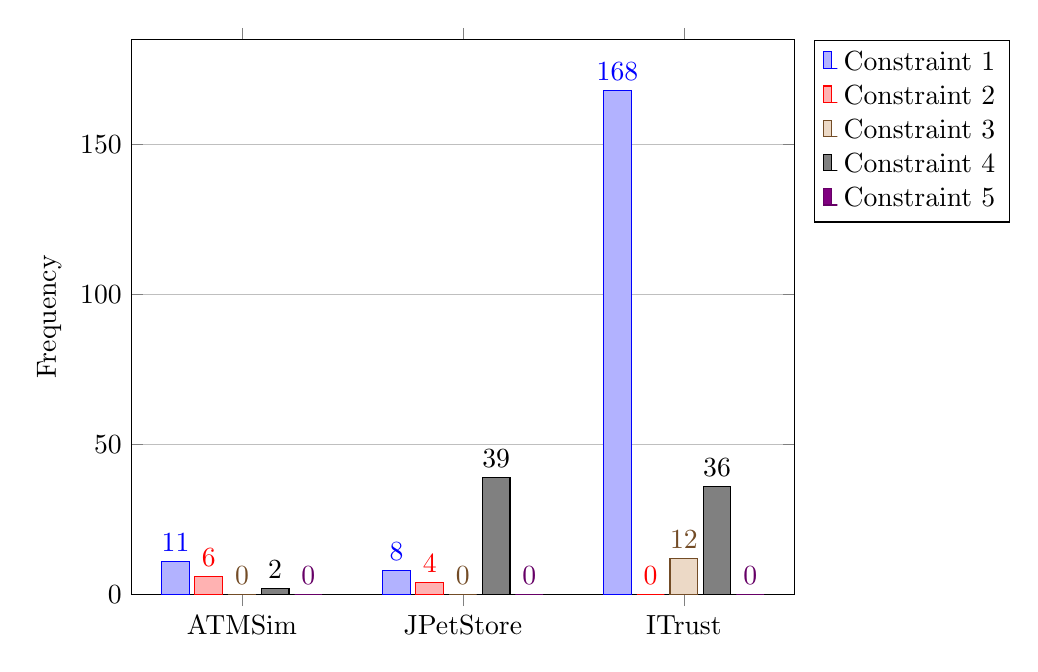
\begin{tikzpicture}
\begin{axis}[
    width=10cm,
    ybar,
    ymin = 0,
    ymajorgrids = true,
    enlarge x limits=0.25,
    xbar legend,
    legend pos=outer north east,
    ylabel={Frequency},
    symbolic x coords={ATMSim,JPetStore,ITrust},
    xtick=data,
    nodes near coords,
    nodes near coords align={vertical},
    ]
%C1
\addplot coordinates {(ATMSim,11) (JPetStore,8) (ITrust,168)};
%C2
\addplot coordinates {(ATMSim,6) (JPetStore,4) (ITrust,0)};
%C3
\addplot coordinates {(ATMSim,0) (JPetStore,0) (ITrust,12)};
%C3
\addplot coordinates {(ATMSim,2) (JPetStore,39) (ITrust,36)};
%C3
\addplot coordinates {(ATMSim,0) (JPetStore,0) (ITrust,0)};
\legend{Constraint 1,Constraint 2,Constraint 3, Constraint 4, Constraint 5}
\end{axis}
\end{tikzpicture}

\caption{The frequency of constraint violations found in the three projects.}
\label{bar:frequency_violation_compraison}
\end{figure}